\documentclass[tikz,border=2pt]{standalone}
\usepackage{tikz}
\usetikzlibrary{positioning}
\begin{document}
% Namikawa--Ueno type: II^*-II^*_l
% Target MRNC type: II^*_{lD}
% Adapted from Tim Dokchitser picture: II^*_{{\it n}D}
% Parameter substitution: n -> l
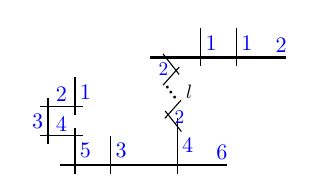
\begin{tikzpicture}[xscale=0.57,yscale=0.62]
\draw[thick,shorten >=2] (4/15,0)--(395/96,0) node[inner sep=2pt,blue,above left,scale=0.8] {6};
\draw[shorten <=-3pt, shorten >=-3pt] (3/5,0)--node[inner sep=2pt,scale=0.8,blue,right] {5} (3/5,3/5);
\draw[shorten <=-3pt, shorten >=-3pt] (3/5,3/5)--node[inner sep=2pt,scale=0.8,blue,above] {4} (0,3/5);
\draw[shorten <=-3pt, shorten >=-3pt] (0,3/5)--node[inner sep=2pt,scale=0.8,blue,left] {3} (0,6/5);
\draw[shorten <=-3pt, shorten >=-3pt] (0,6/5)--node[inner sep=2pt,scale=0.8,blue,above] {2} (3/5,6/5);
\draw[shorten <=-3pt] (3/5,6/5)--node[inner sep=2pt,scale=0.8,blue,right] {1} (3/5,9/5);
\draw[shorten <=-3pt] (7/5,0)--node[inner sep=2pt,scale=0.8,blue,right] {3} (7/5,3/5);
\draw[shorten <=-3pt, shorten >=-3pt] (461/160,0)--node[inner sep=2pt,scale=0.8,blue,right] {4} (461/160,4/5);
\draw (461/160,4/5) 
    ++(0.09,-0.11)--++(-0.36,0.42)++(0.16,-0.15)  
    ++(0,0.02)
      node[blue,scale=0.7,inner sep=1,anchor=west]{2}
    ++(0,-0.02)
    ++(-0.17,0)--++(0.36,0.37)++(-0.14,0.04)  
    node{$\cdot$} ++(-0.08,0.1) node{$\cdot$}
    ++(-0.08,0.1) node{$\cdot$}++(0.19,-0.06)    node[auto,inner sep=5,scale=0.7,anchor=west]{$l$}
    ++(-0.29,0.13)--++(0.36,0.37)++(-0.19,0)   
    ++(0,-0.04)
      node[blue,scale=0.7,inner sep=1,anchor=east]{2}
    ++(0,0.04)
    ++(0.19,0)++(0,-0.15)--++(-0.36,0.42);
\draw[thick,shorten >=2] (34/15,353/160)--(163/30,353/160) node[inner sep=2pt,blue,above left,scale=0.8] {2};
\draw[shorten <=-3pt] (17/5,353/160)--node[inner sep=2pt,scale=0.8,blue,right] {1} (17/5,449/160);
\draw[shorten <=-3pt] (21/5,353/160)--node[inner sep=2pt,scale=0.8,blue,right] {1} (21/5,449/160);
\end{tikzpicture}
\end{document}
